% !TEX root = ../thesis.tex

\section{Results}
\label{sec:results}
This is the Results section.

\subsection{SOM Metrics}
\label{subsec:results_som_metrics}

\subsubsection{SOM-Induced Quantization}
\label{subsubsec:results_som_quantization}

heat map showing distance?

show quantization error vs. training duration

show influence of learning rate

kernel radius?

what about influence of alpha?

\subsubsection{Vector-Node Count}
\label{subsubsec:results_vector_node_count}

\subsubsection{Map Emptiness}
\label{subsubsec:results_map_emptiness}

\begin{figure}[!htb]
  \centering
\begin{subfigure}{0.45\textwidth}
  \centering
  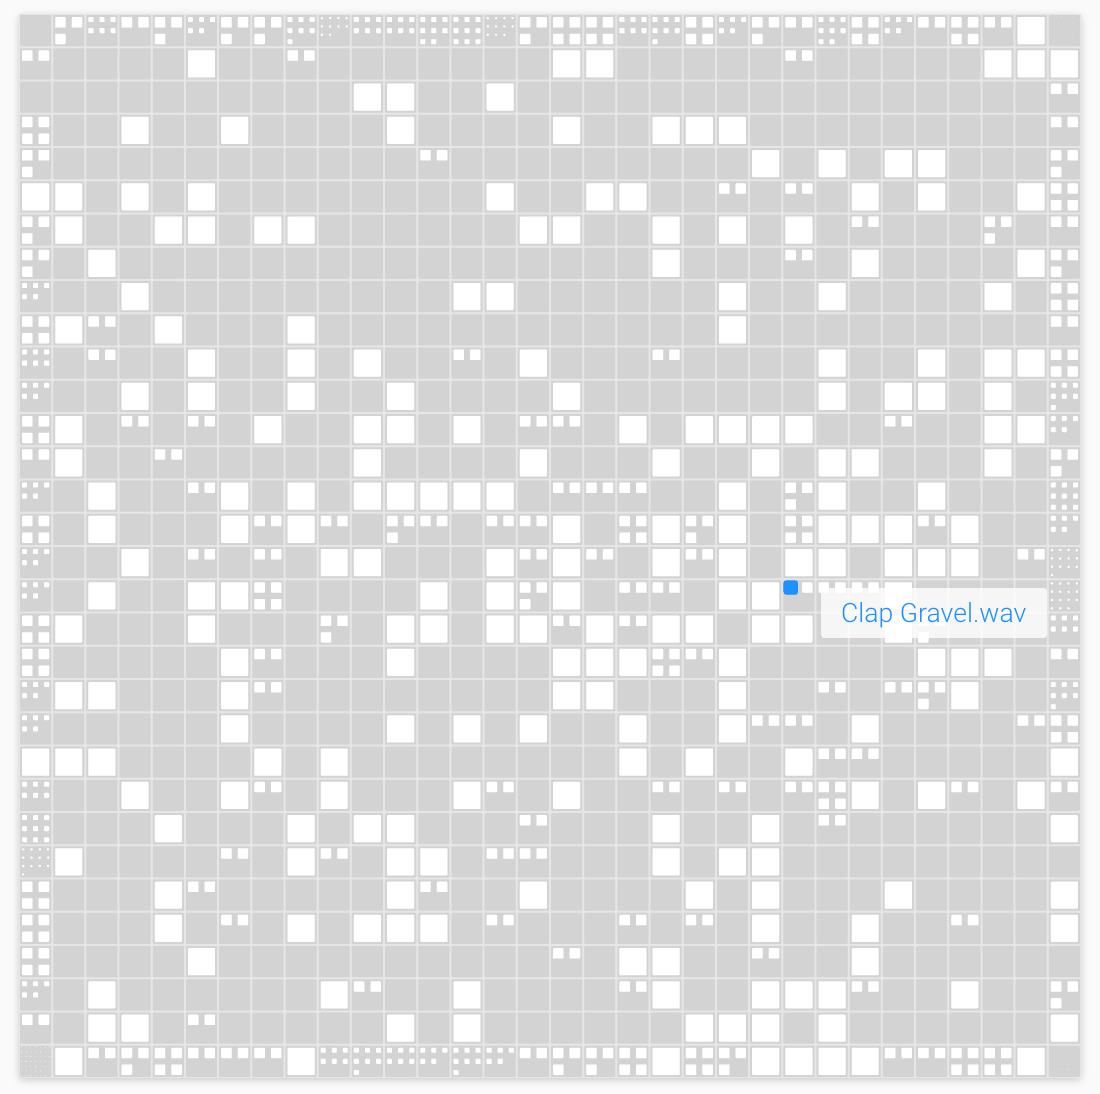
\includegraphics[width=\textwidth]{SOM-Browser_no-FNP}
  \caption{\textit{SOM Browser} without \gls{fnp}}
  \label{fig:results_no_fnp}
\end{subfigure}
~
\begin{subfigure}{0.45\textwidth}
  \centering
  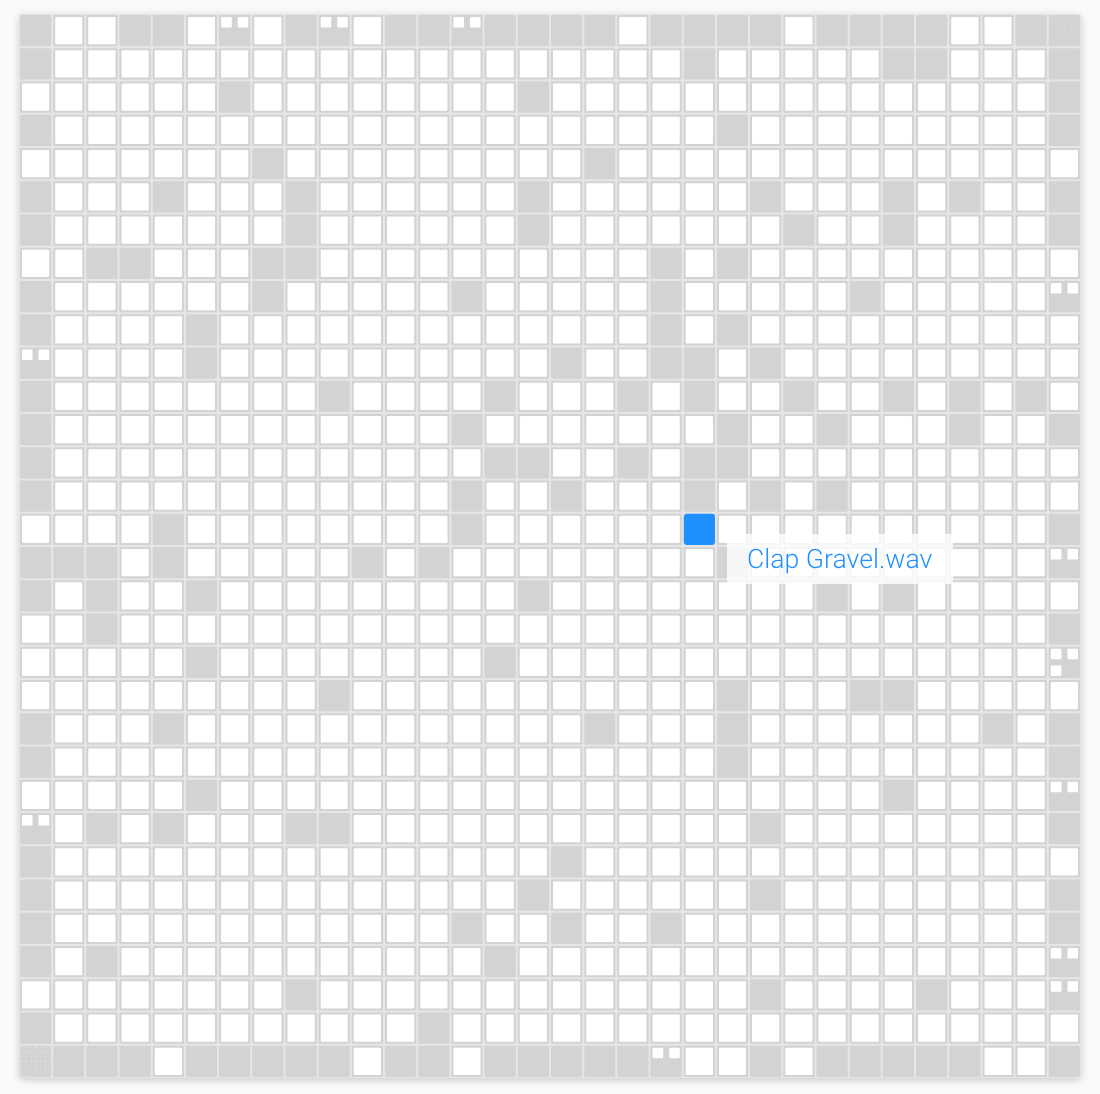
\includegraphics[width=\textwidth]{SOM-Browser_FNP}
  \caption{\textit{SOM Browser} with \gls{fnp}}
  \label{fig:results_fnp}
\end{subfigure}
\caption[\textit{SOM Browser}: Influence of FNP on Map Emptiness]
{\textit{SOM Browser}: Influence of FNP on Map Emptiness for the
\textit{Drum Essentials} sample library}
\label{fig:results_fnp_comparison}
\end{figure}


\subsection{Interview Results}
\label{subsec:results_interview}
The group of interview subjects consisted of one woman and four men with an
average age of 36 years and an average 15 years of experience in the audio
industry. Subjects described their profession as one or several of the
following: composer, producer, DJ, performer, sound / mixing engineer, sound
designer.

\bigskip

Subject responses to the ratings questions described in Section
\ref{subsubsec:questions_used} can be found in Figure \ref{fig:results_ratings}.

\bigskip

Recordings of the conducted interviews were transcribed by the author. These
transcriptions were examined for instances relating to the interview questions
and the relevant instances marked and subsequently coded using an
\textit{emergent coding} approach \citep[p.304]{lazar2017}. These codes are
presented here using matrix data displays (\citet[p.254]{saldana2015},
\citet{henwood2003}).

\clearpage

\begin{figure}[!hp]
  \centering
  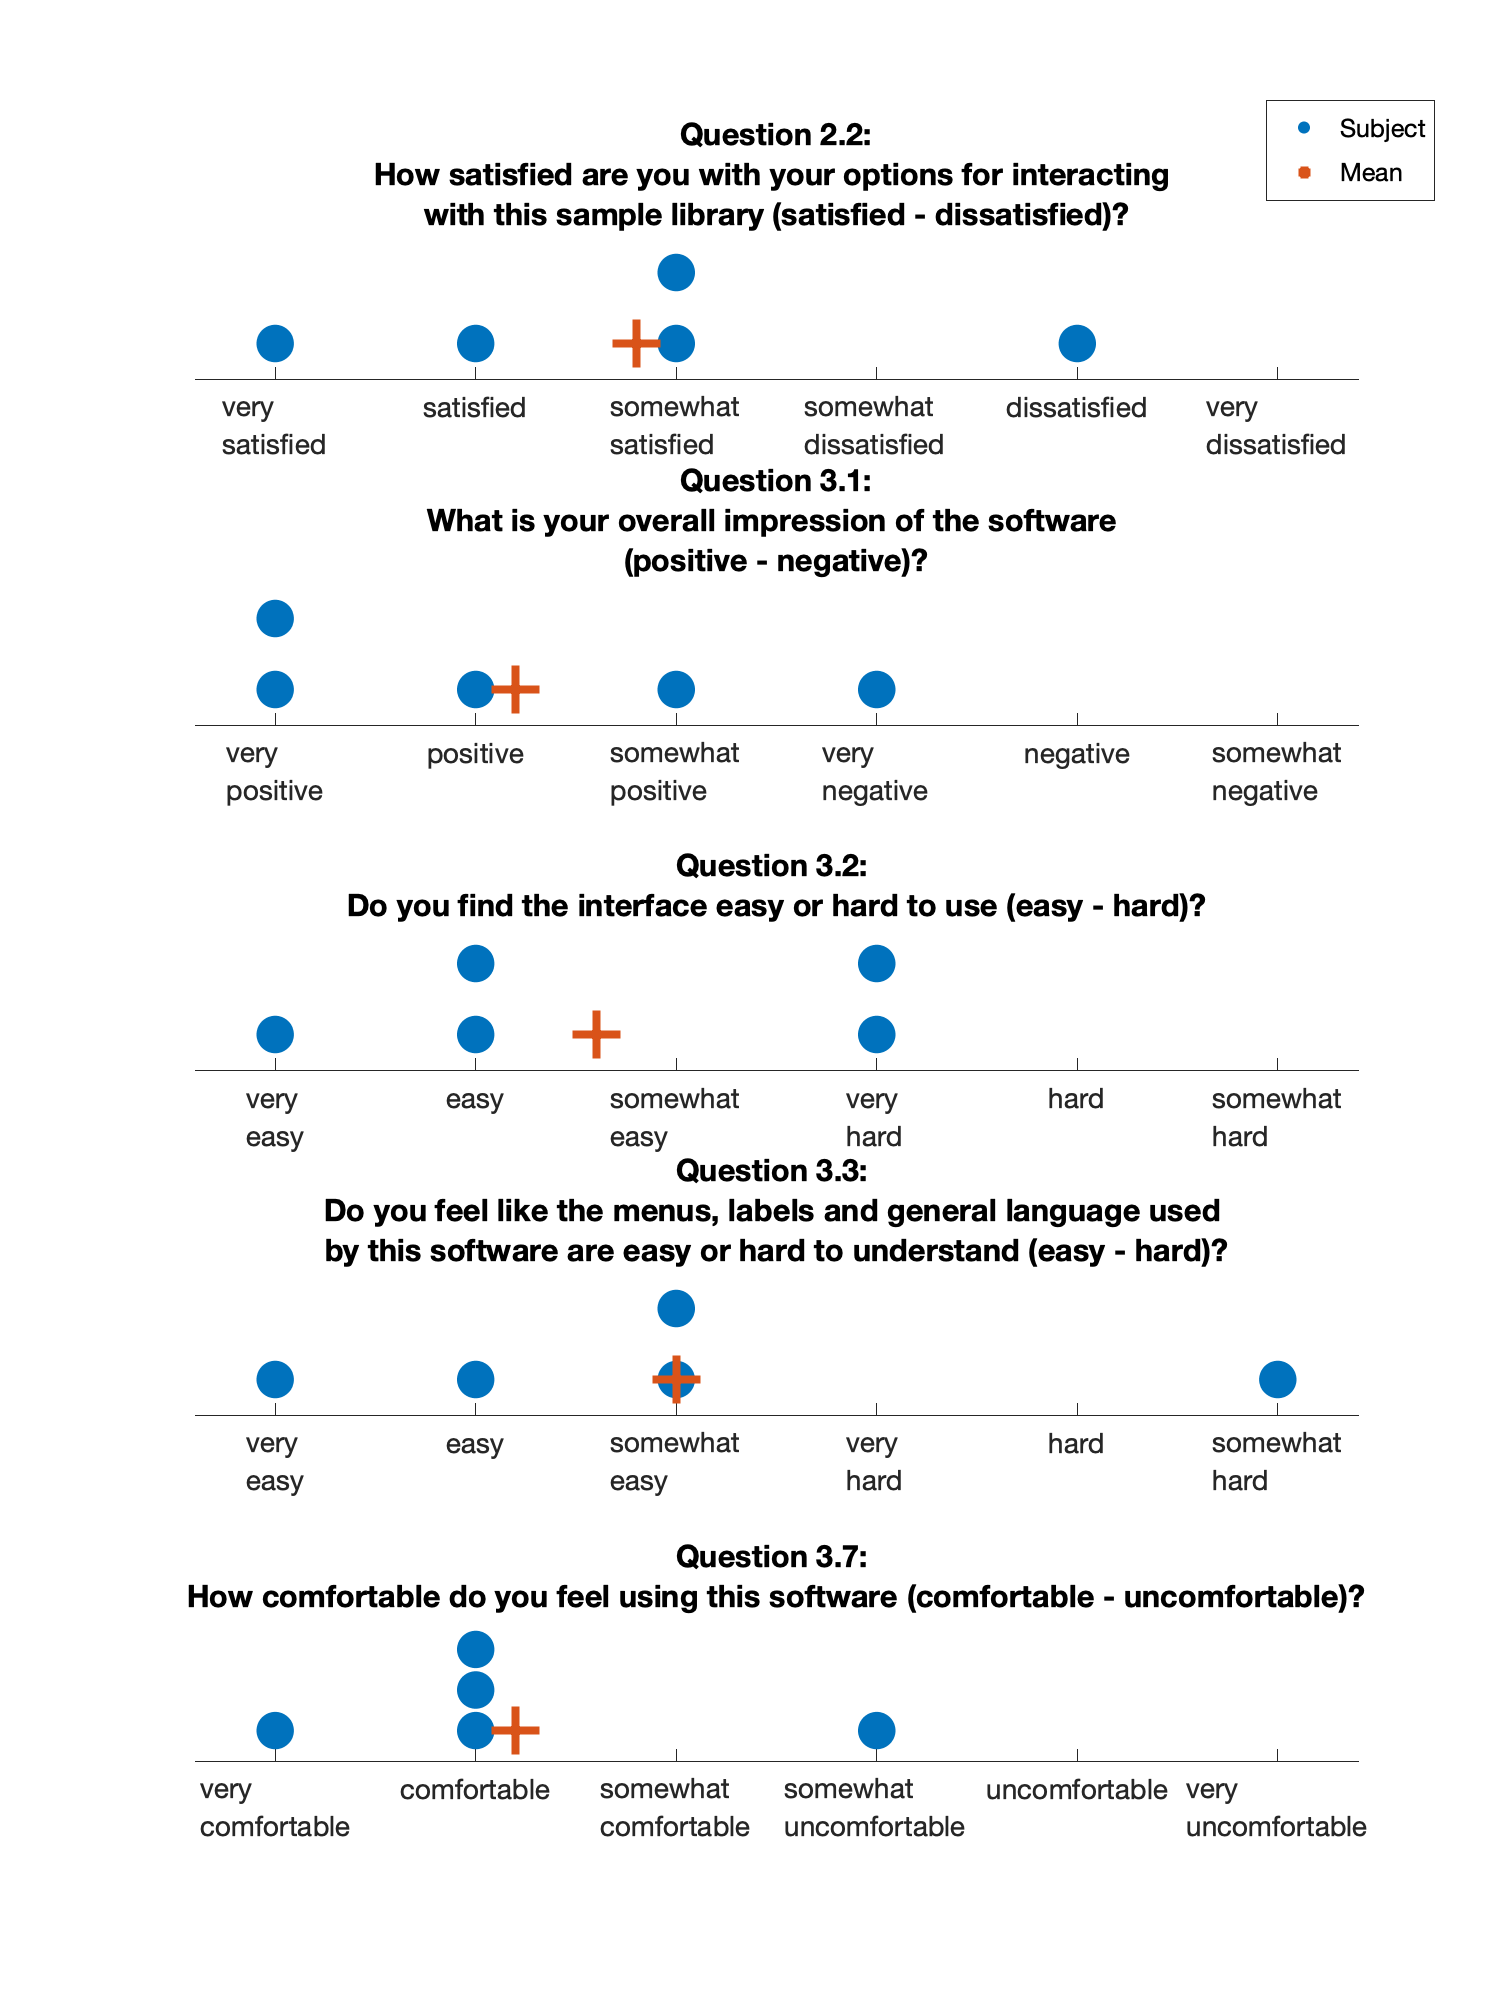
\includegraphics[width=\linewidth, trim = 25mm 10mm 10mm 10mm, clip]
  {eval_ratings}
  \caption[Interview Ratings]{Likert scale ratings by interview subjects for
  questions concerning satisfaction with their current sample library workflow
  and first \textit{SOM Browser} impressions}
  \label{fig:results_ratings}
\end{figure}

\clearpage

\subsubsection{Established Workflow Responses}
\label{subsubsec:results_established_workflow}
Sections 1 and 2 of the interview questionnaire inquire about subjects' current
workflow practices. Recorded responses are grouped into the categories
\textit{Description} (see Table \ref{table:current_workflow_description}) and
\textit{Assessment} (see Table \ref{table:current_workflow_assessment}). A
flowchart of established workflow practices was extracted from these responses
and is displayed in Figure \ref{fig:results_current_workflow}.

\begin{table}[!htb]
  \renewcommand{\arraystretch}{1.2}
  \centering
  \textbf{Description of Established Sample Library Workflow} \\ [3mm]
  \footnotesize
  \colorbox{light-bg}{
  \begin{tabular}{ p{4.0cm} p{4.75cm} p{4.75cm} }
  \hline
    \textbf{Code} & \textbf{Example} & \textbf{Summary} \\
    \hline
    \textbf{Mental Representation}
    &
    "I know exactly what I'm looking for"
    &
    Subjects often have a clear \textbf{mental representation} of the sound they
    are searching.
    \\
    \textbf{Goal Pursuit}
    &
    [I listen to sounds] "[u]ntil I find the one that I want"
    &
    Subjects will only look for sounds until they find something that satisfies
    their immediate needs.
    \\
    \textbf{Search Algorithm}
    &
    "I would just go through every folder [...] and listen carefully to every
    sound"
    &
    Subjects describe three \textbf{search "algorithms"}: sequential
    (listening in alphabetical order), name-based (looking at file or subfolder
    names) and random search (arbitrarily selecting samples).
    \\
    \textbf{Contextual Evaluation}
    &
    "quickly go through the sounds while the track is playing and then find
    one that kind of fits"
    &
    The ability to audition sounds in the \textbf{context} of the relevant
    project is important.
    \\
    \textbf{Iteration}
    &
    "I will have like eight different kick drums [...] and then I go through
    them again as another iteration of choice."
    &
    Subjects will select a variety of samples as potential candidates and then
    perform another search among the selected subset.
    \\
    \textbf{Frustration}
    &
    "it takes a lot of time actually and it's not the most fun part"
    &
    Looking through lists of samples sequentially is perceived to cause
    \textbf{frustration}.
    \\
  \end{tabular}}
  \caption[Established Sample Library Workflow Description: Response Codes]
  {Established sample library workflow as described by subjects. Shown are
  response codes along with example data and interpretive summary.}
  \label{table:current_workflow_description}
\end{table}

\pagebreak

\begin{figure}[!htb]
  \centering
  \textbf{Established Sample Library Workflow} \\ [5mm]
  \begin{tikzpicture}[node distance=3mm,
    box/.style={
      rectangle, text centered, rounded corners,
      minimum width = 5cm, minimum height = 2cm,
      fill=table-bg-two, text width=5cm
    },
    item/.style={
      rectangle, text centered, rounded corners, font=\footnotesize,
      minimum width = 3cm, minimum height = 1cm,
      fill=table-bg-two, text width=3cm
    },
    arrow/.style={
      thick,->,>=stealth
    }
  ]
  % \tikzstyle{every node}=[font=\footnotesize]

  \node (well_defined) [item] {Well-Defined};
  \node (ambiguous) [item, below = of well_defined] {Ambiguous};
  \node (os) [item, below = 6mm of ambiguous] {\gls{os} File Browser};
  \node (daw) [item, below = of os] {\gls{daw} Browser};
  \node (sequential) [item, below = 6mm of daw] {Sequential};
  \node (name_based) [item, below = of sequential] {Name-Based};
  \node (random) [item, below = of name_based] {Random};
  \node (match) [item, below = 6mm of random] {Match};
  \node (iteration) [item, below = of match] {Iteration};

  \path (well_defined.west)-- coordinate (aux1) (ambiguous.west);
  \node (mental_representation) [box, left = 6mm of aux1]
  {Mental Representation \\of Sound};

  \path (os.west)-- coordinate (aux2) (daw.west);
  \node (tool) [box, left = 6mm of aux2] {Search Tool};

  \node(algorithm) [box, left = 6mm of name_based] {Search Algorithm};

  \path (match.west)-- coordinate (aux3) (iteration.west);
  \node (evaluation) [box, left = 6mm of aux3] {Contextual Evaluation};

  \draw [arrow] (mental_representation) -- (tool);
  \draw [arrow] (tool) -- (algorithm);
  \draw [arrow] (algorithm) -- (evaluation);

  \draw [arrow] (mental_representation) -- (well_defined);
  \draw [arrow] (mental_representation) -- (ambiguous);

  \draw [arrow] (tool) -- (os);
  \draw [arrow] (tool) -- (daw);

  \draw [arrow] (algorithm) -- (evaluation);
  \draw [arrow] (algorithm) -- (sequential);
  \draw [arrow] (algorithm) -- (name_based);
  \draw [arrow] (algorithm) -- (random);

  \draw [arrow] (evaluation) -- (match);
  \draw [arrow] (evaluation) -- (iteration);

  \node (ctrl1) [below = 1cm of iteration, anchor = south] {};
  \node (ctrl2) [below left = 1cm of evaluation, anchor = north] {};
  \node (ctrl3) [left = 9mm of algorithm, anchor = west] {};
  % HOLY $#&* THIS ARROW WAS A STRUGGLE TO GET STRAIGHT
  \draw [dashed, arrow] (iteration.south) -- (ctrl1.north) -- (ctrl2.east) --
  (ctrl3.east) -- (algorithm);
\end{tikzpicture}
\caption[Established sample library workflow]{Flowchart of established sample
library workflow as described by interview subjects}
\label{fig:results_current_workflow}
\end{figure}

\begin{table}[!htb]
  \renewcommand{\arraystretch}{1.2}
  \centering
  \textbf{Description of Established Sample Library Workflow} \\ [3mm]
  \footnotesize
  \colorbox{light-bg}{
  \begin{tabular}{ p{4.0cm} p{4.75cm} p{4.75cm} }
  \hline
    \textbf{Code} & \textbf{Example} & \textbf{Summary} \\
    \hline
    \textbf{Requires Organization}
    &
    "if I was organized and I had my 5000 sounds from the past five years it
    [would] be really nice"
    &
    Subjects note that their current workflow relies on sample libraries that
    are organized in some way and note sources of \textbf{frustration} such as
    lost or duplicate files.
    \\
    \textbf{Requires Experience}
    &
    "experience [...] is probably the key"
    &
    \textbf{Experience} (both in a general professional sense and specific to
    the sample libraries at hand) is mentioned as a factor for an efficient,
    successful workflow.
    \\
    \textbf{Good Enough}
    &
    "It could be better but it's okay. Like, it works in most of cases."
    &
    Current workflow practices are deemed \textbf{"good enough"}, but subjects
    are interested in alternative approaches.
    \\
    \textbf{Time-Consuming}
    &
    "[H]ow to listen to all this?"
    &
    Subjects remark upon the amount of time and effort that go into searching
    through sample libraries.
    \\
    \textbf{Overwhelming}
    &
    "it was overwhelming [...] to look through all this"
    &
    Finding relevant samples in a library is described as \textbf{overwhelming}.
    \\
    \textbf{Alphabetic Bias}
    &
    "I think it makes no sense that I'm mainly choosing from the first half of
    the alphabet"
    &
    Sample selection is influenced by alphabetical name ordering. Typically,
    samples positioned towards the beginning of an alphabetical list are more
    likely to be chosen.
    \\
  \end{tabular}}
  \caption[Established Sample Library Workflow Assessment: Response Codes]
  {Subjects' assessment of established sample library workflow. Shown are
  response codes along with example data and interpretive summary.}
  \label{table:current_workflow_assessment}
\end{table}

\pagebreak



\subsubsection{SOM Browser Responses}
\label{subsubsec:results_som-browser_responses}
The third and largest section of the questionnaire assesses subjects' first
impressions of the \textit{SOM Browser} software. Responses varied between
individual subjects, but can generally be grouped into \textit{positive} and
\textit{negative} statements. These are presented in Tables
\ref{table:responses_som-browser_positive} and
\ref{table:responses_som-browser_negative}. Notable \textit{positive} responses
were prompted by the \textbf{visual design} of the software, as well as the
creative potential for using the software as an \textbf{instrument} because of
the \textbf{gestural interaction} it facilitates.

\begin{table}[!htb]
  \renewcommand{\arraystretch}{1.2}
  \centering
  \textbf{SOM Browser: Positive Responses} \\ [3mm]
  \footnotesize
  \colorbox{light-bg}{
  \begin{tabular}{ p{4.0cm} p{4.75cm} p{4.75cm} }
  \hline
    \textbf{Code} & \textbf{Example} & \textbf{Summary} \\
    \hline
    \textbf{Visual Design}
    &
    "Visually, it makes sense."
    &
    Subjects characterize the \textbf{visual design} of the software as
    appealing.
    \\
    \textbf{Gestural Interaction}
    &
    "for expressive gestures as a performance tool, it’s fantastic as a
    continuous thing"
    &
    Continuous playback with trackpad/mouse gestures (while holding down Shift)
    is seen positively when using \textit{SOM Browser} more like an instrument.
    \\
    \textbf{App as Instrument}
    &
    "this is an instrument"
    &
    Subjects remark upon potential creative use of the software by not just
    using it to select samples, but also treating it as an \textbf{instrument}
    by itself.
    \\
    \textbf{User-Friendly}
    &
    "Even if I would be starting, like, it's not confusing, [...] it’s clear"
    &
    Subjects describe use of the software as \textbf{user-friendly}.
    \\
    \textbf{Favorites Selection}
    &
    "I also find the favorites pretty good"
    &
    The \textit{Favorites} bar at the bottom of \textit{SOM Browser} can be seen
    as positive.
    \\
  \end{tabular}}
  \caption[\textit{SOM Browser}: Positive Responses]{Positive responses given
  by subjects after using \textit{SOM Browser}. Shown are response codes along
  with example data and interpretive summary.}
  \label{table:responses_som-browser_positive}
\end{table}

\begin{table}[!htb]
  \renewcommand{\arraystretch}{1.2}
  \centering
  \textbf{SOM Browser: Negative Responses} \\ [3mm]
  \footnotesize
  \colorbox{light-bg}{
  \begin{tabular}{ p{4.0cm} p{4.75cm} p{4.75cm} }
  \hline
    \textbf{Code} & \textbf{Example} & \textbf{Summary} \\
    \hline
    \textbf{Incomprehensible Map Organization}
    &
    "I don't get the order, that’s frustrating."
    &
    Subjects are not able to discern any logical order within the map.
    \\
    \textbf{Usefulness}
    &
    "right now it's beautiful but it makes no sense unfortunately"
    &
    Subjects question the \textbf{usefulness} of the software in its current
    state.
    \\
    \textbf{Confused by Empty Nodes}
    &
    "Why are there a few grayed out?"
    &
    Empty nodes on the map confuse subjects.
    \\
    \textbf{Overwhelming}
    &
    "looking at these many, many tiny squares gives me anxiety"
    &
    The map interface is seen by some subjects as \textbf{overwhelming}.
    \\
    \textbf{No File Labels}
    &
    "here it’s just white bricks"
    &
    The fact that no files besides the current selection are labelled on the map
    is seen negatively by some subjects.
    \\
    \textbf{Unnecessary Interface Elements}
    &
    "Eliminate the top bar, eliminate all the bottom just keep this [points to
    map in center]"
    &
    Subjects question the need for interface elements besides the central map
    display.
    \\
  \end{tabular}}
  \caption[\textit{SOM Browser}: Negative Responses]{Negative responses given
  by subjects after using \textit{SOM Browser}. Shown are response codes along
  with example data and interpretive summary.}
  \label{table:responses_som-browser_negative}
\end{table}



\subsubsection{Workflow Comparison: SOM Browser vs. Established Workflow}
\label{subsubsec:workflow_comparison}
Response codes concerning the comparison of \textit{SOM Browser} and established
workflows are shown in Table \ref{table:responses_workflow_comparison}. Subjects
stated a clear preference for their established workflows, but remarked upon the
\textbf{potential} of the software, particularly if it could be presented as an
\textbf{optional workflow} that integrates with existing production environments
(something that is echoed in the feature requests in Section
\ref{subsubsec:feature_requests}).

\begin{table}[!htb]
  \renewcommand{\arraystretch}{1.2}
  \centering
  \textbf{Workflow Comparison: SOM Browser vs. Established Workflow} \\ [3mm]
  \footnotesize
  \colorbox{light-bg}{
  \begin{tabular}{ p{4.0cm} p{4.75cm} p{4.75cm} }
    \hline
    \textbf{Code} & \textbf{Example} & \textbf{Summary} \\
    \hline
    \textbf{Preference for Established Workflow}
    &
    "I wouldn't want to miss my old way of looking for stuff."
    &
    Subjects state a preference for their established way of working with
    samples.
    \\
    \textbf{Optional Workflow}
    &
    "I would go for the traditional and just be presented with this like [an]
    alternative"
    &
    Subjects would like to incorporate \textit{SOM Browser} into their workflow
    if it was well-integrated into their existing tools and could be used as an
    alternative view mode.
    \\
    \textbf{Potential}
    &
    "I could imagine, that this if you use it a bit and you get used to it,
    yeah, it could make things faster actually"
    &
    The potential for certain workflow improvements such as increased speed and
    removal of alphabetical bias is acknowledged.
    \\
  \end{tabular}}
  \caption[Workflow Comparison \textit{SOM Browser} vs. Established Workflow]
  {Subjects' responses when asked to compare \textit{SOM Browser} to their
  established workflows and state a preference. Shown are response codes along
  with example data and interpretive summary.}
  \label{table:responses_workflow_comparison}
\end{table}


\subsubsection{SOM Browser: Feature Requests}
\label{subsubsec:feature_requests}
Lastly, subjects were asked what changes and additions they would like to see in
the presented software. These responses can be found in Table
\ref{table:responses_feature_requests}. Two particularly noteworthy responses
were the desire for \textbf{\gls{daw} integration} of the functionality of
\textit{SOM Browser} and the ability to navigate the map using
\textbf{Arrow keys}.

\begin{table}[!htb]
  \renewcommand{\arraystretch}{1.2}
  \centering
  \textbf{SOM Browser: Feature Requests} \\ [3mm]
  \footnotesize
  \colorbox{light-bg}{
  \begin{tabular}{ p{4.0cm} p{4.75cm} p{4.75cm} }
    \hline
    \textbf{Code} & \textbf{Example} & \textbf{Summary} \\
    \hline
    \textbf{\gls{daw} Integration}
    &
    "I would really like to see it as a plug-in or inserted in the production
    environment that I have. I would definitely not use, it if it's a
    standalone thing."
    &
    Subjects want to \textbf{integrate} the functionality of
    \textit{SOM Browser} into their established production environment, either
    in plug-in form or directly within the \gls{daw}.
    \\
    \textbf{Arrow Key Navigation}
    &
    "You need the arrows."
    &
    The need for granular map navigation using the keyboard's
    \textbf{Arrow keys} was mentioned repeatedly by subjects.
    \\
    \textbf{User-Definable Map Organization}
    &
    "be able to choose what each axis is"
    &
    The ability to more explicitly control how maps are organized.
    \\
    \textbf{Pre-Categorization}
    &
    "a pre-categorization would be nice"
    &
    Subjects express the wish to incorporate some sort of
    \textbf{categorization} to precede map calculation into the software.
    \\
    \textbf{File Limit}
    &
    "it’s about limiting the squares"
    &
    Subjects would like to \textbf{limit} the total number of files that can be
    displayed on a map. By preventing larger maps, the interface would
    potentially become less overwhelming.
    \\
    \textbf{Multi-Page Maps}
    &
    "[...] something that’s like a page based. Like, you go through the folders
    or you just type in quickly, just give here all the kicks or only all the
    snares"
    &
    Larger sample libraries could be spread out across several \textbf{pages},
    potentially based on the previously mentioned \textbf{pre-categorization}.
    \\
    \textbf{Feature Filters}
    &
    "[If] I'm looking for a sample that [...] is very short, then you
    would have to be able to filter this somehow"
    &
    Incorporate the option to \textbf{filter} samples on the map based on
    certain feature values or ranges.
    \\
    \textbf{Color Coding}
    &
    "all the dark and bass heavy stuff [...] in another color than [...] all the
    tsh-tsh-tsh stuff [makes high frequency noises]"
    &
    Introduce \textbf{color} as an additional dimension to display information
    about the files on the map.
    \\
    \textbf{Touchscreen Support}
    &
    "Only if it's like on a touchscreen"
    &
    Support for \textit{SOM Browser} on \textbf{touchscreen} devices.
    \\
    \textbf{Color Customization}
    &
    "maybe people can choose their colors"
    &
    Give users the option to \textbf{customize} interface \textbf{colors}.
    \\
    \textbf{Sample Retriggering}
    &
    "when I'm on a square I need a way to retrigger"
    &
    Ability to trigger the same sample repeatedly without clicking multiple
    times (presumably by pressing the Spacebar).
    \\
    \textbf{Larger Font Size}
    &
    "the letters [need] to be a bit more prominent"
    &
    Increase font sizes across the interface.
    \\
  \end{tabular}}
  \caption[SOM Browser: Feature Requests]{Subjects' feature requests for
  \textit{SOM Browser}. Shown are response codes along with example data and
  interpretive summary.}
  \label{table:responses_feature_requests}
\end{table}
